\section{Data Analysis of Study}
As discussed, the participants had to fill out a small questionnaire every day in the evening and these answers were then matched against the computed results.

\subsection{Calculating the Answers}
The answers had to be converted into scalars such that they could be compared directly to the computed features. 

In any case the feature calculation closest to the answer was used, prioritising a features calculated after the given answer, rather than earlier.

Homestay: Use the time of sending in the answer as the elapsed time. If the user is 'out' at the time of answering, they will likely taken this into account.

Routine index: Transform scale to routine index, i.e. scale $s \in \{0, 1, 2, 3, 4, 5\}$, then the routine index is calculated as $r = \frac{s}{s_{max}}$



\subsection{Error Measuring}

Regarding data collection, figure \ref{fig:plot-megabytes} displays how much data was collected per participant which gives an indication of how much could be computed. It also became clear that some participants did not collect nearly as much data as others, and because of this their results are expected to be worse.


\begin{figure}
    \centering
    \includegraphics[width=\textwidth]{example-image-a}
    \includegraphics[width=\textwidth]{example-image-b}
    \caption{The storage space required in MB for the raw GPS data (top) and the stops (bottom) for each participant. There are clear discrepancies in the amount of data collected by each user}
    \label{fig:plot-megabytes}
\end{figure}

Discussion of Compression of GPS to stops, for the researcher. i.e place saved by compressing dataset to stops


\begin{figure}
    \centering
    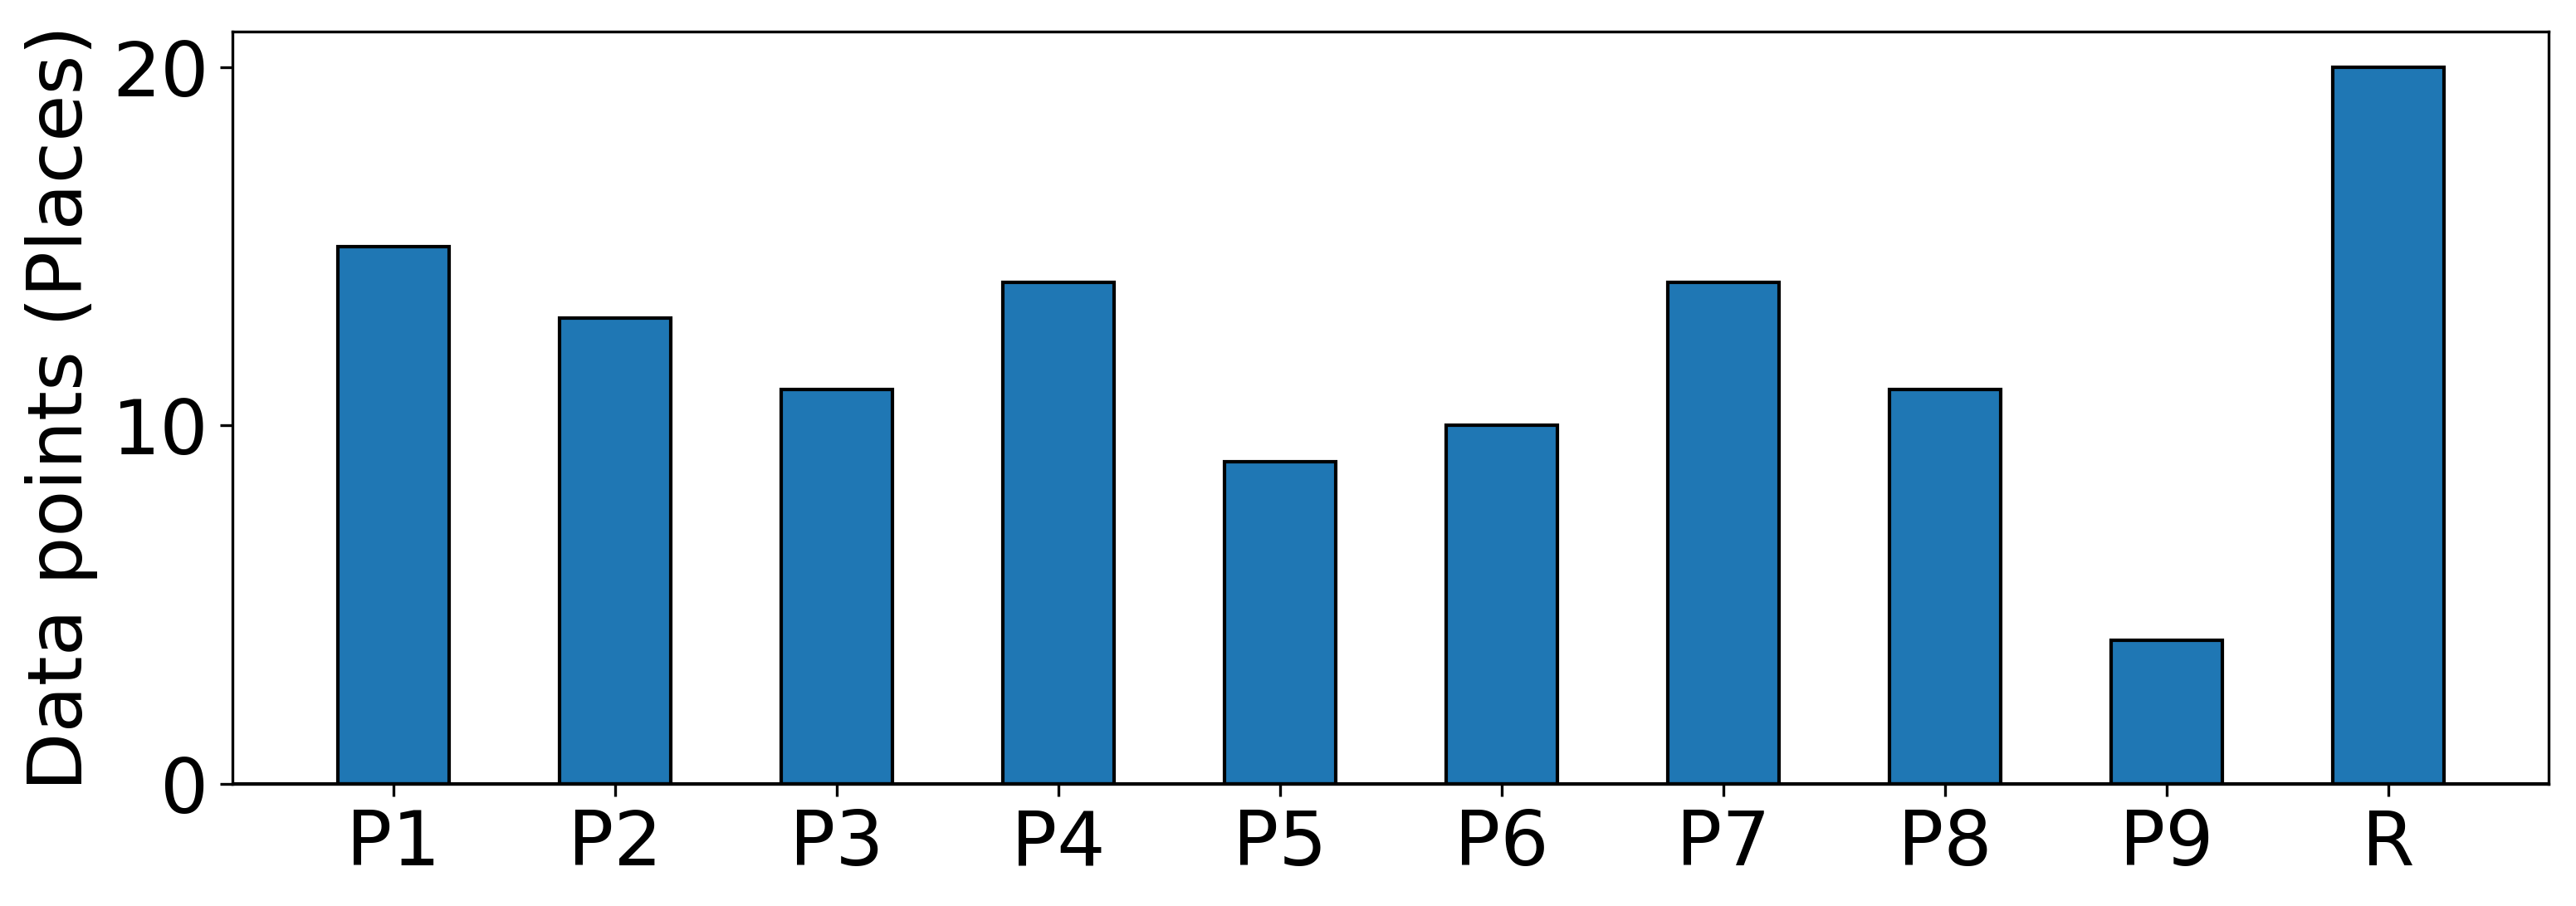
\includegraphics[0.5\textwidth]{images/study/n_places.png}
    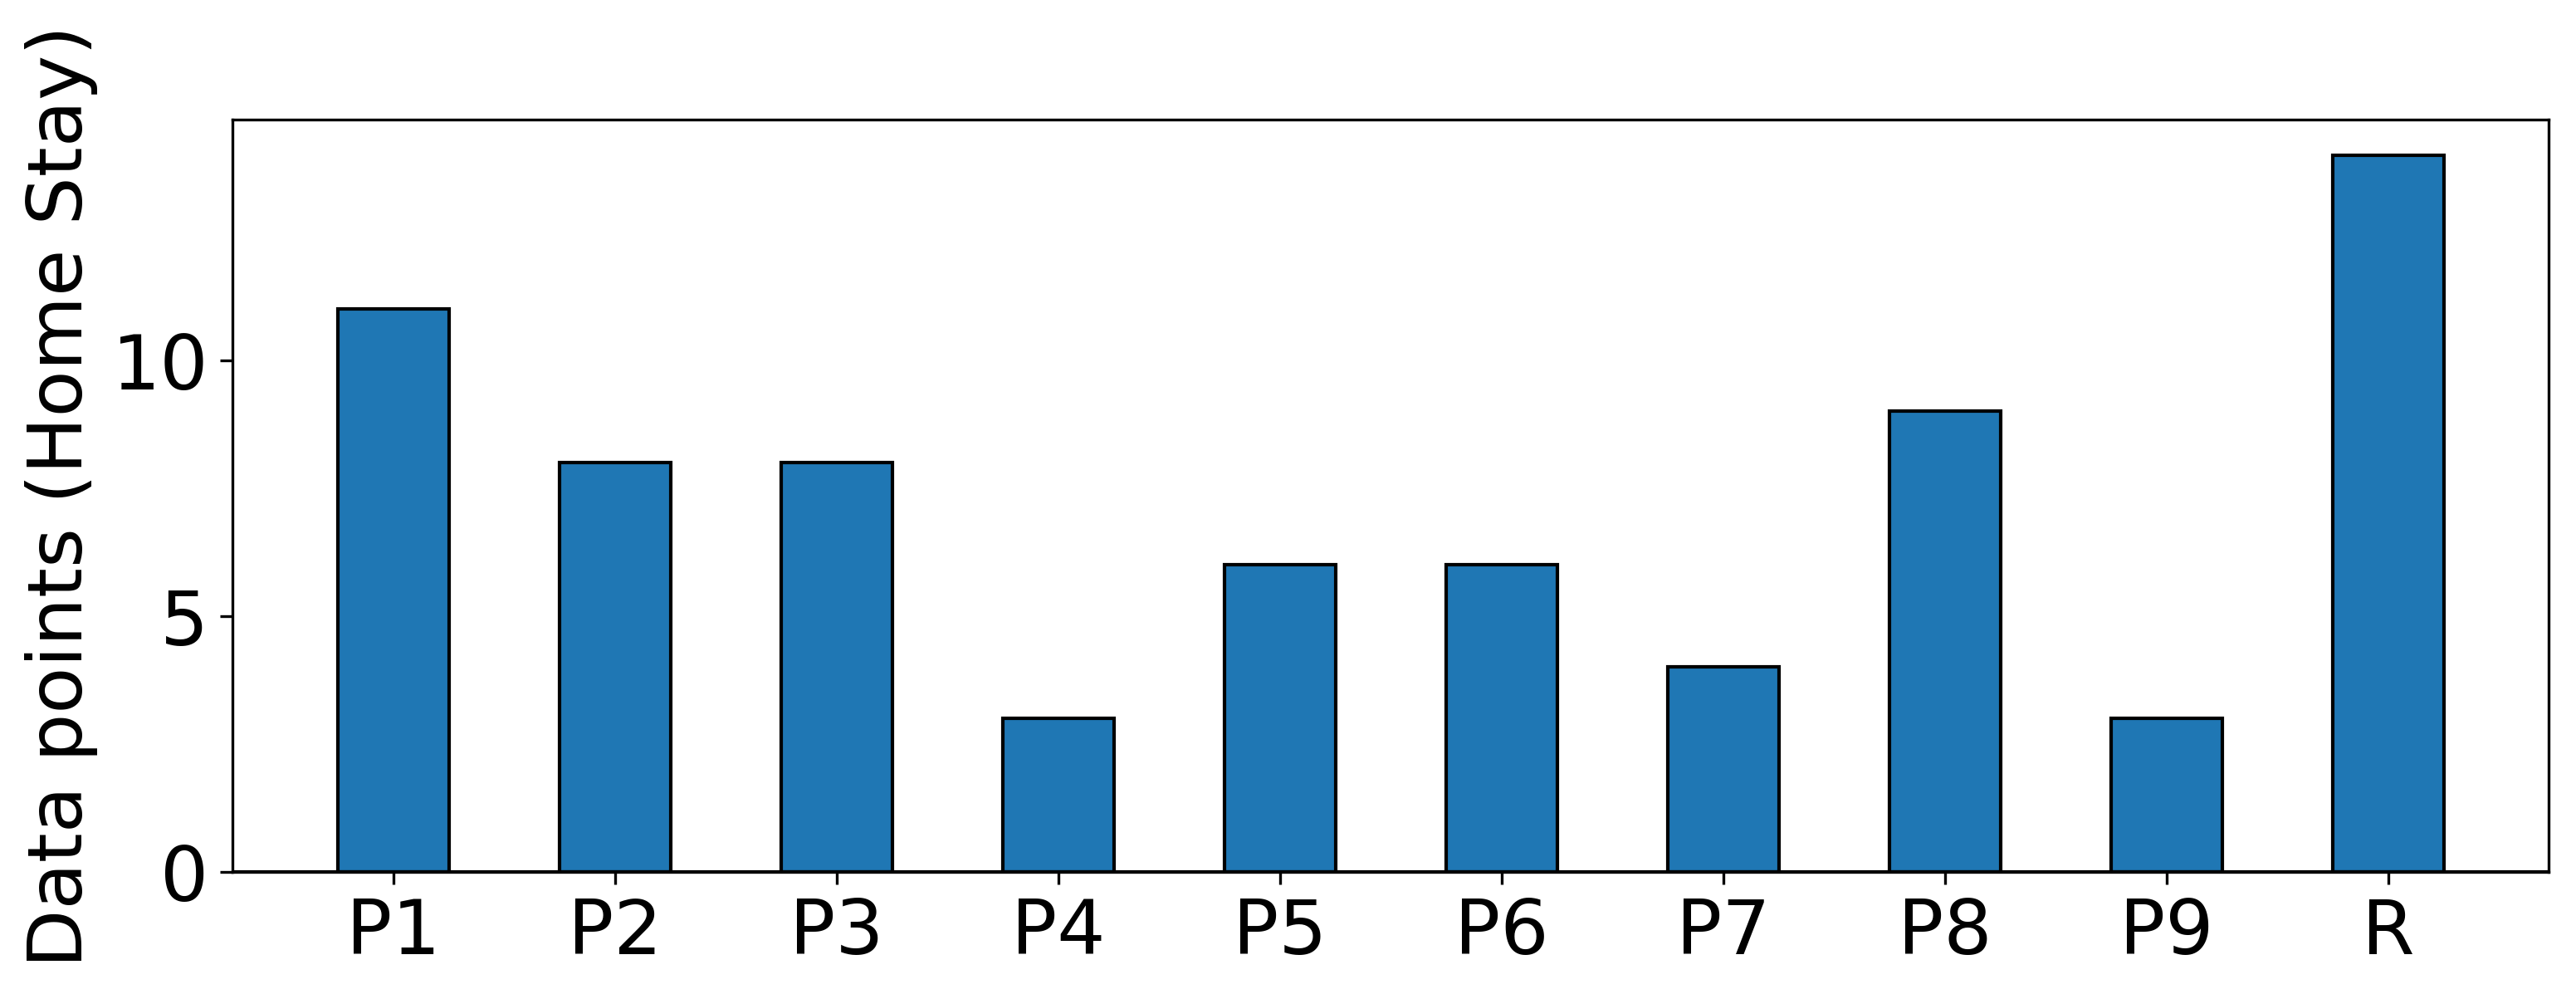
\includegraphics[0.5\textwidth]{images/study/n_homestay.png}
    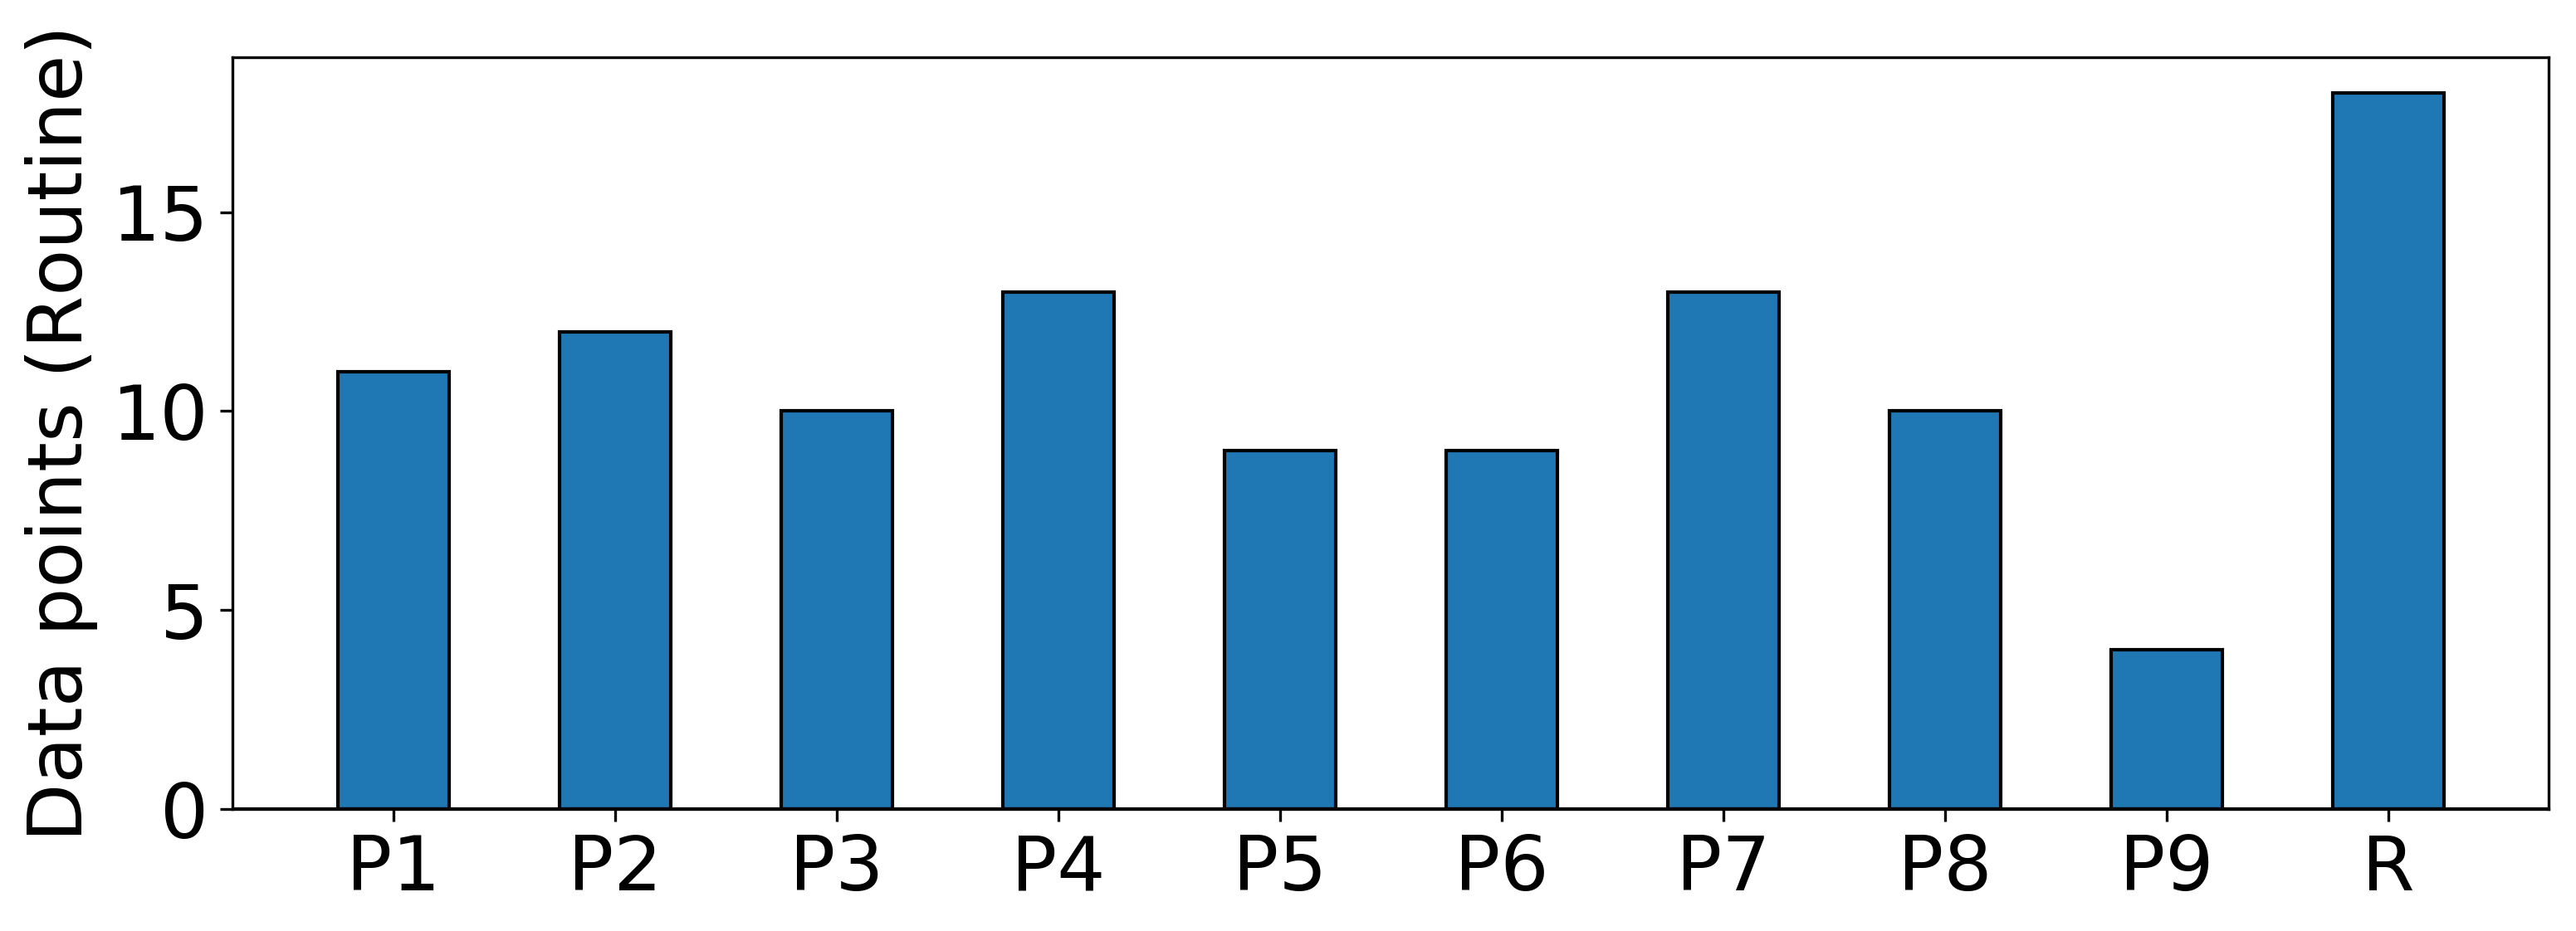
\includegraphics[0.5\textwidth]{images/study/n_routine.png}
    \caption{The number of valid days for each participant}
    \label{fig:plot-daily}
\end{figure}

\begin{figure}
    \centering
    \includegraphics[width=\textwidth]{example-image-a}
    \caption{The storage space required in MB for the raw GPS data (top) and the stops (bottom) for each participant. There are clear discrepancies in the amount of data collected by each participant}
    \label{fig:plot-megabytes}
\end{figure}


The day-by-day results for the author are displayed in figure \ref{fig:plot-daily}.


\begin{figure}
    \centering
    \includegraphics[width=\textwidth]{example-image-a}
    \caption{The number of days where answers weren't given, for each participant.}
    \label{fig:plot-no-answer}
\end{figure}

The number of valid days for a specific feature is a day for which the user gave answers, and the feature could be calculated. If the user for example turned off their phone during the night, the home stay feature could not be calculated, but the routine index feature and the number of places will likely still have been calculated.


\subsection{Subjectivity of Answers and Ground Truth}
A thing to keep in mind is that the participants' answers are not ground truth, and there are multiple reasons why a participants answer may be inaccurate. Firstly, people's subjective recollection is not necessarily as accurate as they think it might me. Secondly, it was not communicated explicitly to the participants what exactly counts as a place, and how their 'routine' is calculated - this means that participants may have filled out the questionnaire differently, given the same ground truth data - for example whether or not being in the garden counts as being home. Secondly, some users misunderstood the routine scale and users whose data looked strange were contacted afterwards to enquire about whether they had misunderstood the question and if so the answers were corrected as much as could be done. Lastly, the hour away from home and routine index answers were very course grained, and therefore the participants were probably rarely able to give exact answers, according to the their own recollection. 

\subsection{Missing Data and Correcting Data}
Some users have a very high amount of missing days regarding answers and data computed. For the Home Stay feature it was required that the user tracked their location during the night from 00:00 to 06:00 and thus if they did not, then the home stay feature could not be evaluated. In addition, some users would fill out the questionnaire for day $n$ on day $n+1$ during the night which resulted in the answers having the wrong date. This was easy to fix by simply moving all answers given between 00:00 and 06:00 to the previous date which got rid of the problematic data points.

\begin{figure}
    \centering
    \includegraphics[width=\textwidth]{example-image-a}
    \includegraphics[width=\textwidth]{example-image-b}
    \includegraphics[width=\textwidth]{example-image-c}
    \caption{The number of removed days per participant for each feature.}
    \label{fig:plot-megabytes}
\end{figure}

\subsection{Feature Evaluation}
Since the home stay feature is calculated by using the \textit{tracked} time at home, divided by the total time time midnight, it only takes a few minutes of missing data to make the home stay feature undershoot. It is therefore to be expected that this feature will lie somewhat lower than the answer given by the user, given the user did not round up excessively.

Its better to consistently under-shoot, that to oscillate
home stay undershoots often


\begin{figure}
    \centering
    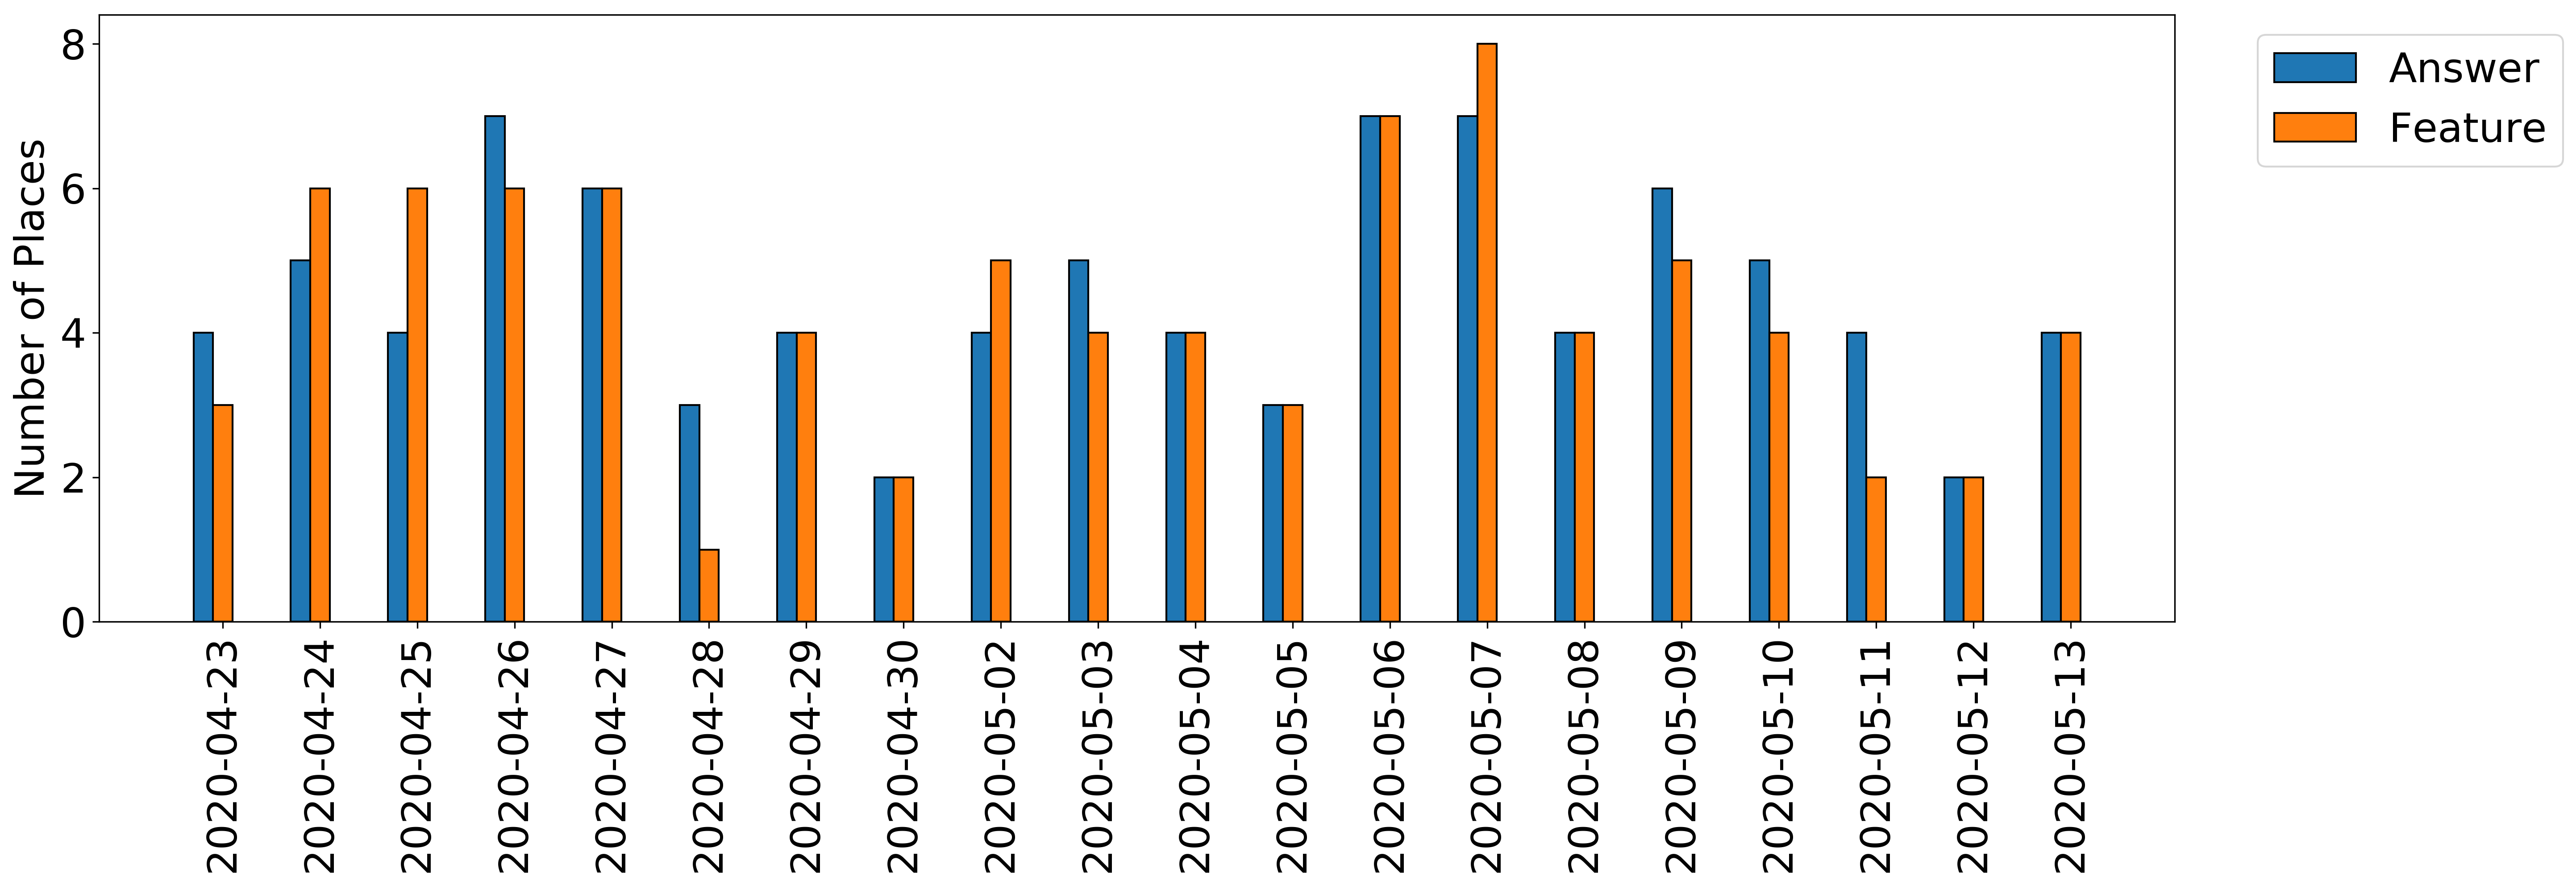
\includegraphics[0.5\textwidth]{images/study/places_d6b2d9b9-398b-4e0d-b52b-224747f515c8.png}
    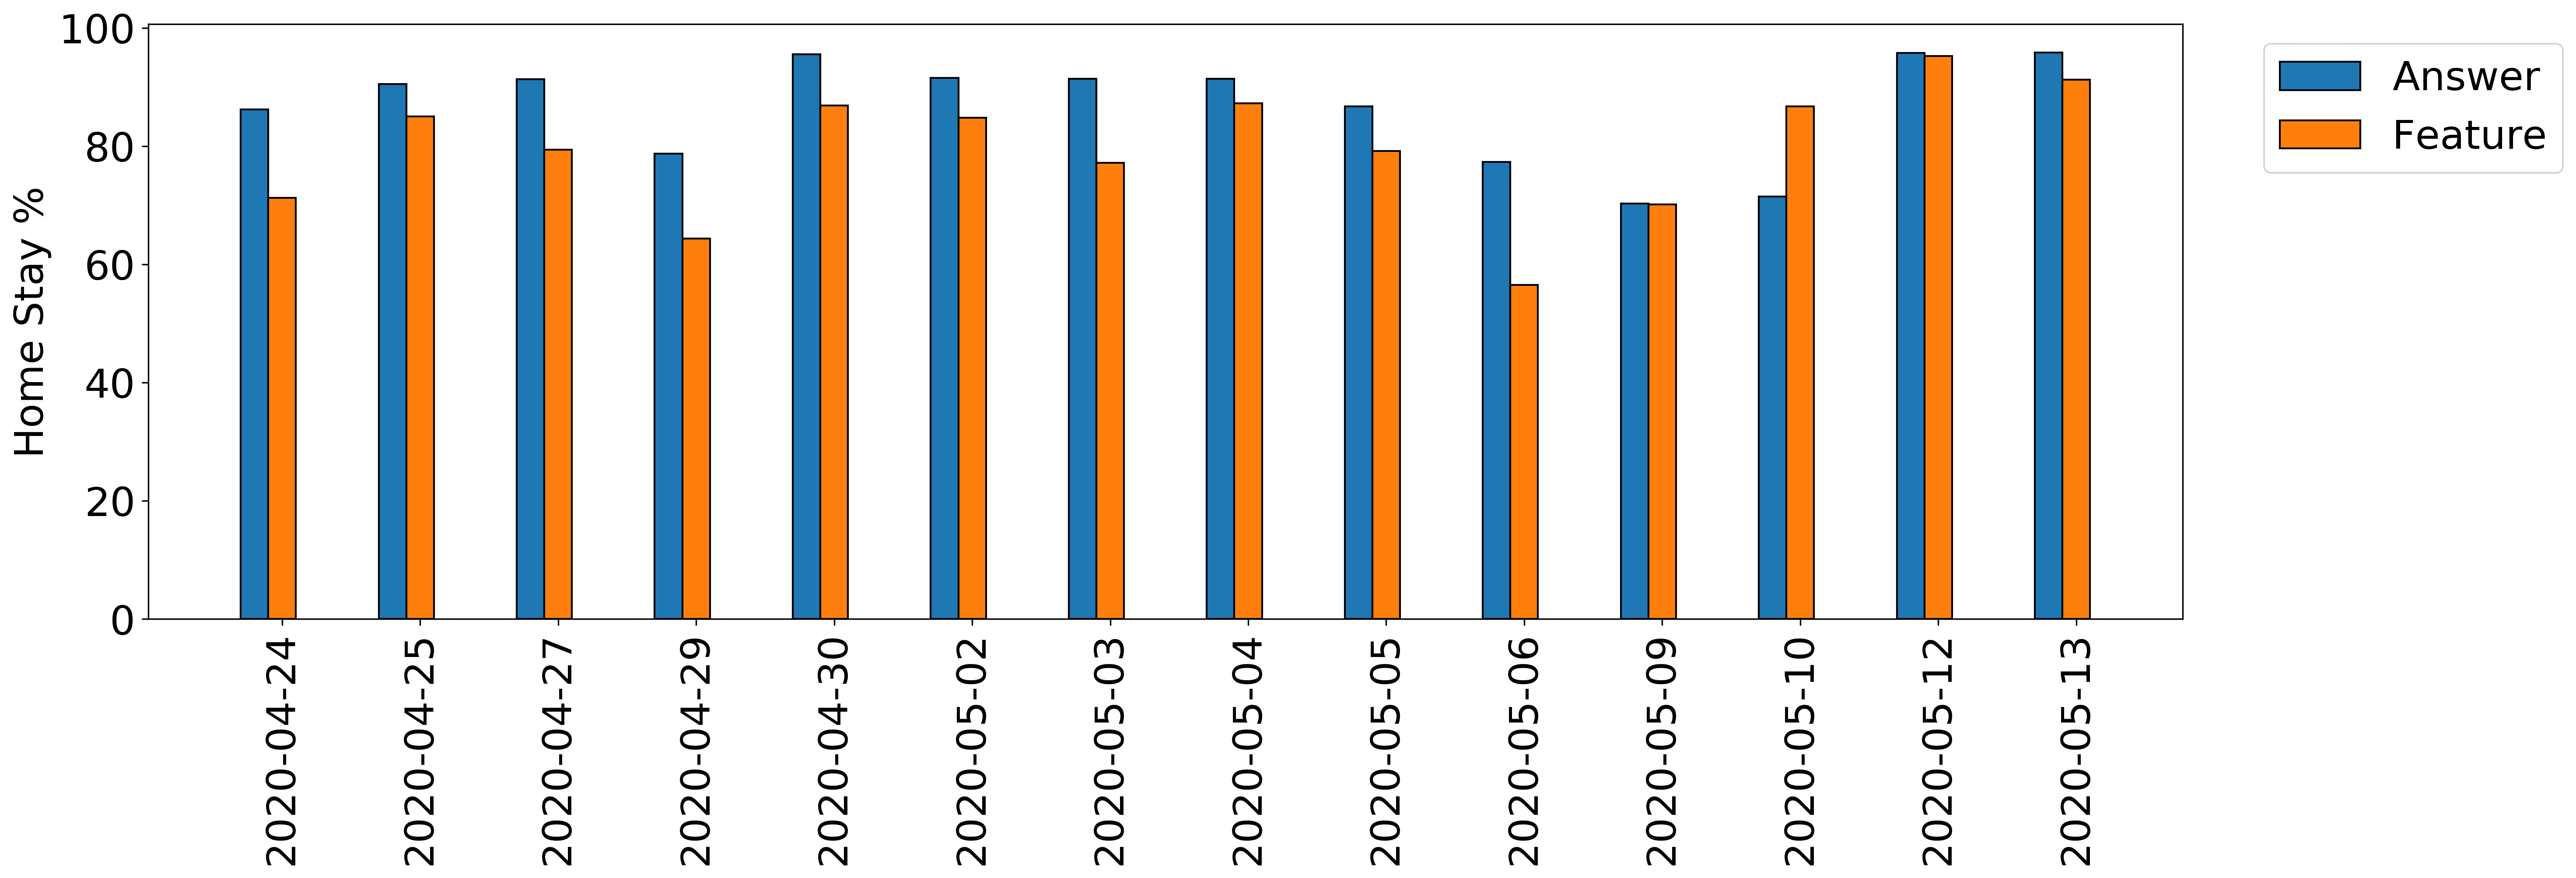
\includegraphics[0.5\textwidth]{images/study/homestay_d6b2d9b9-398b-4e0d-b52b-224747f515c8.png}
    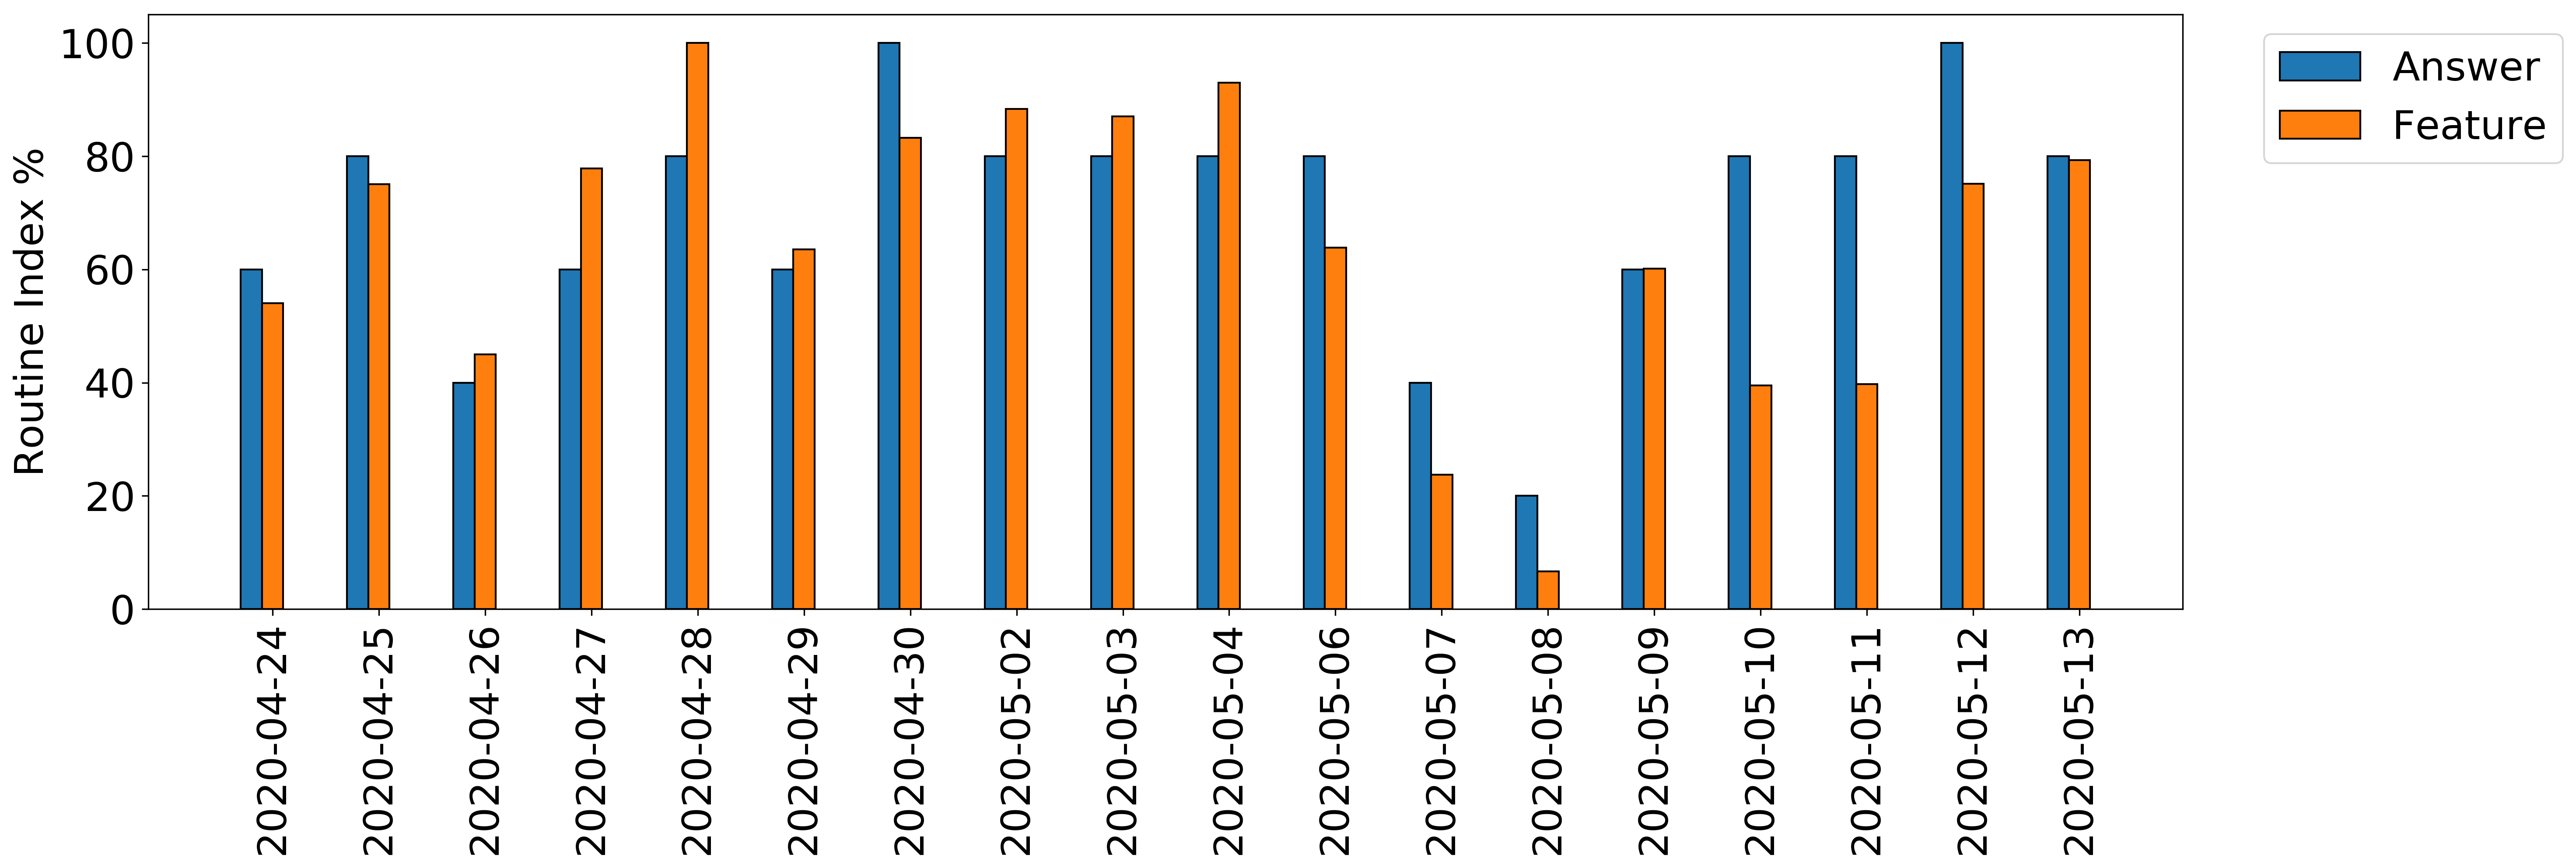
\includegraphics[0.5\textwidth]{images/study/routine_d6b2d9b9-398b-4e0d-b52b-224747f515c8.png}
    \caption{The answered and calculated data for each day, for the author}
    \label{fig:plot-daily}
\end{figure}


\begin{figure}
    \centering
    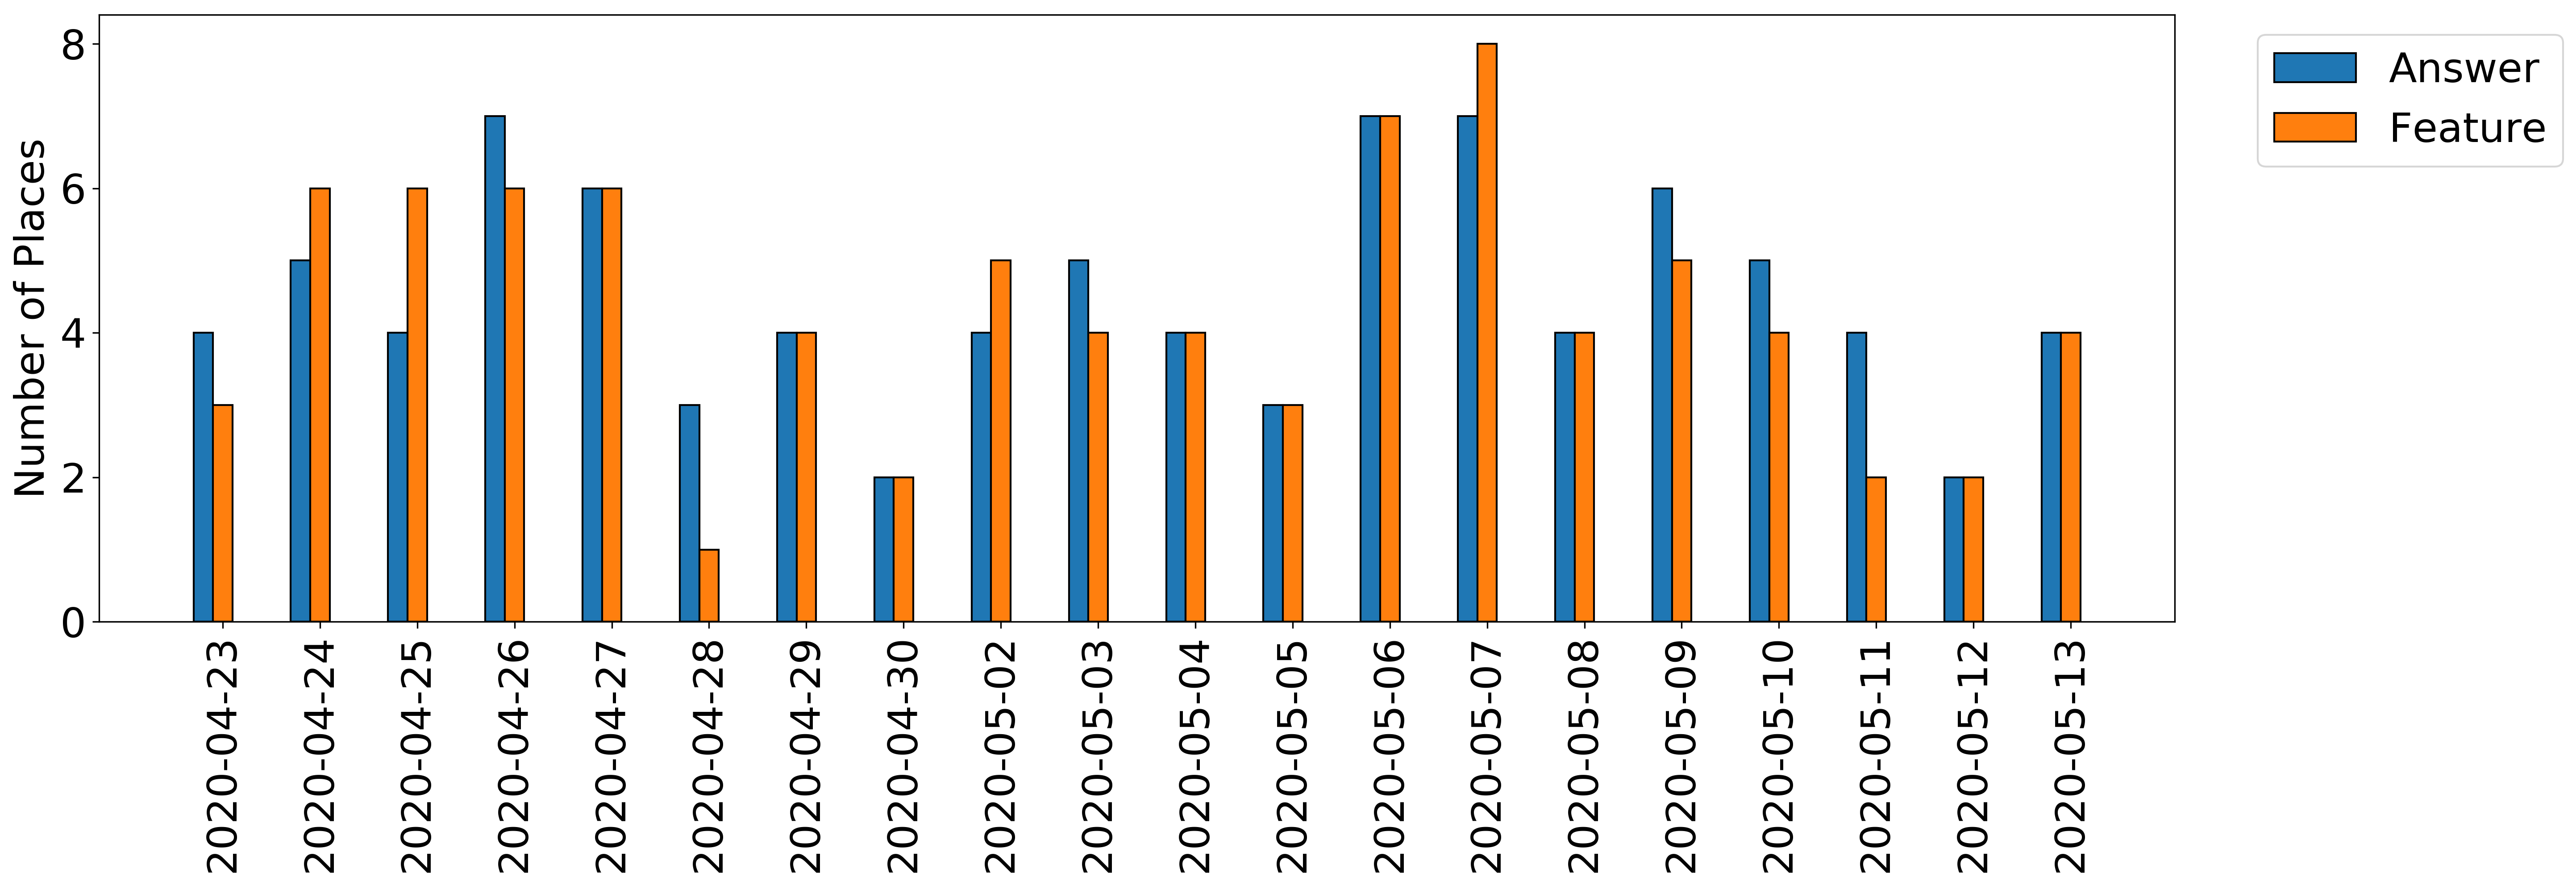
\includegraphics[0.5\textwidth]{images/study/places_d6b2d9b9-398b-4e0d-b52b-224747f515c8.png}
    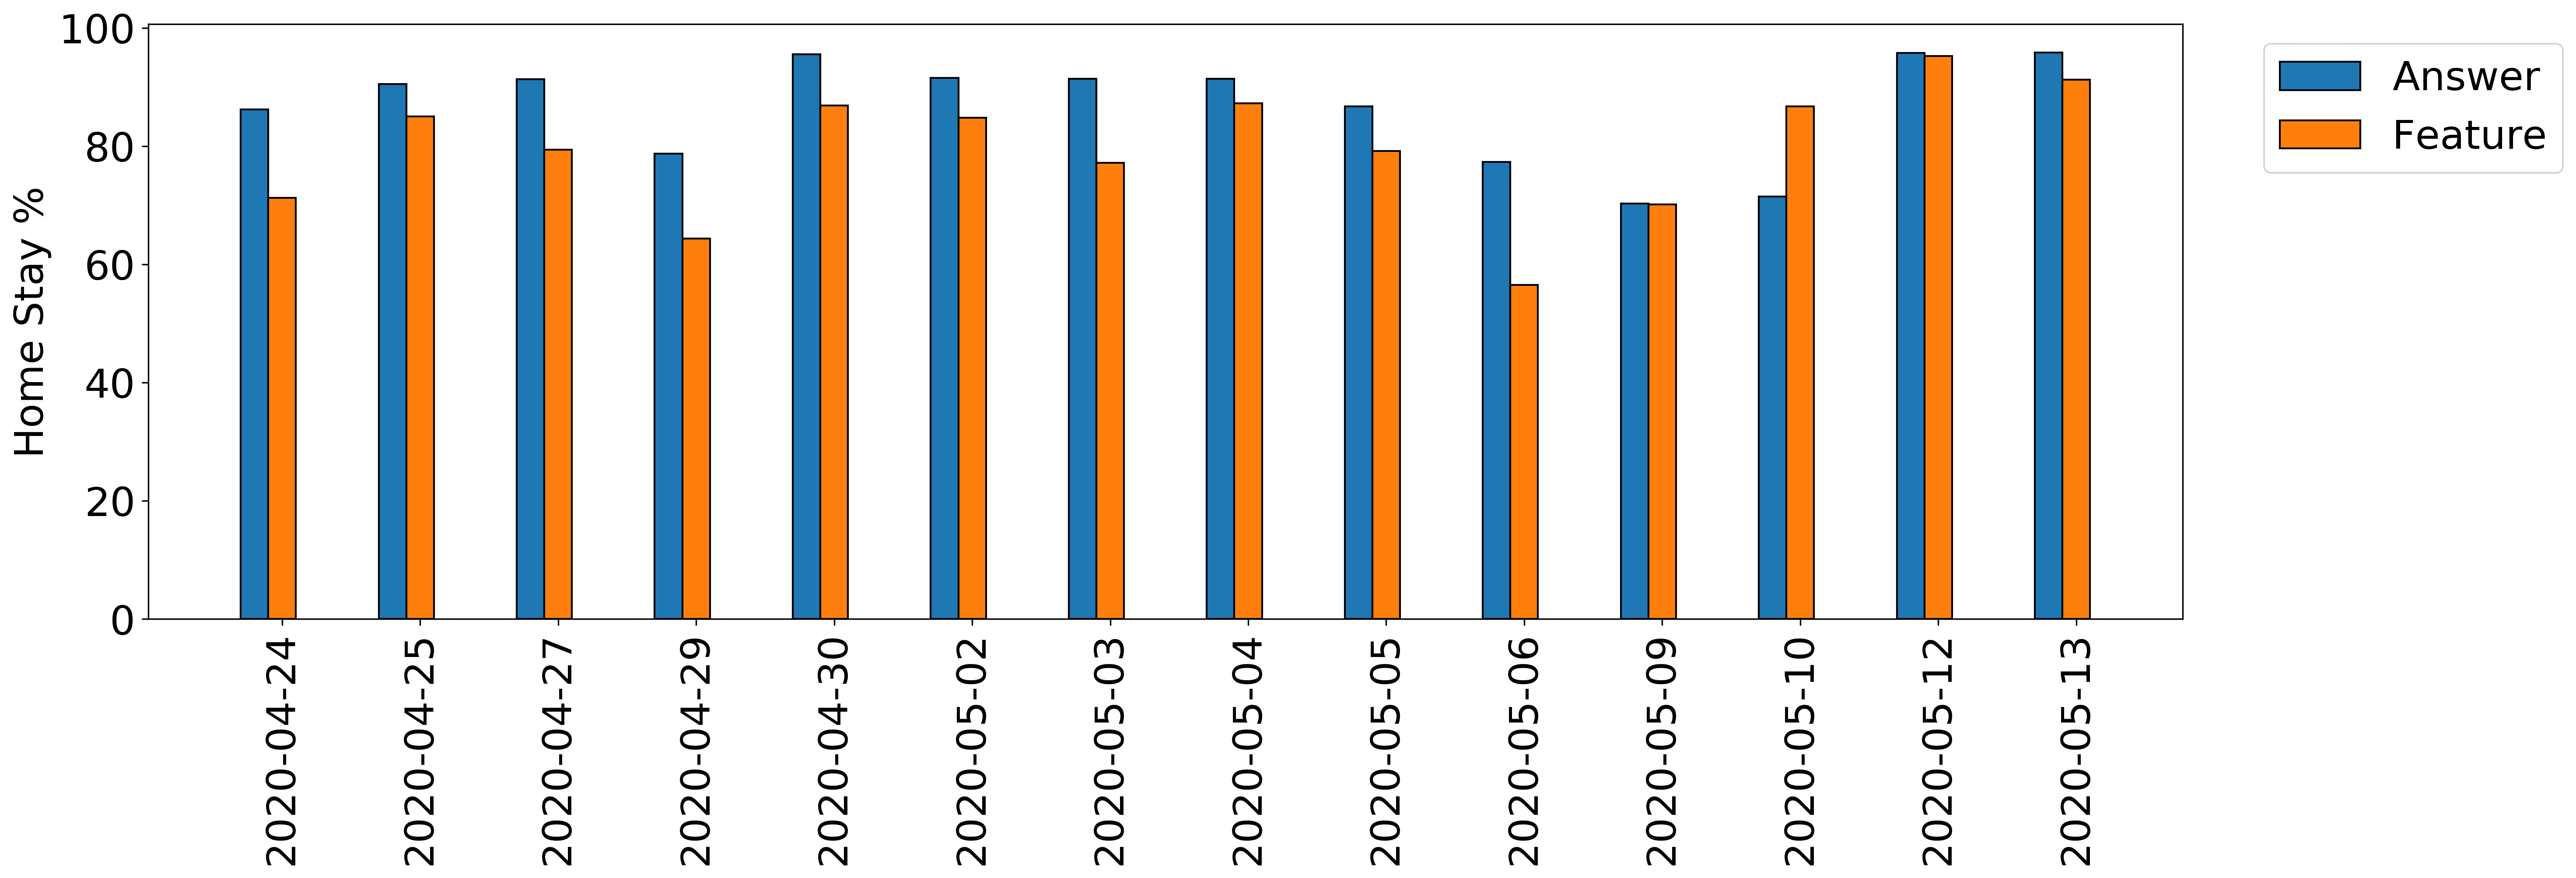
\includegraphics[0.5\textwidth]{images/study/homestay_d6b2d9b9-398b-4e0d-b52b-224747f515c8.png}
    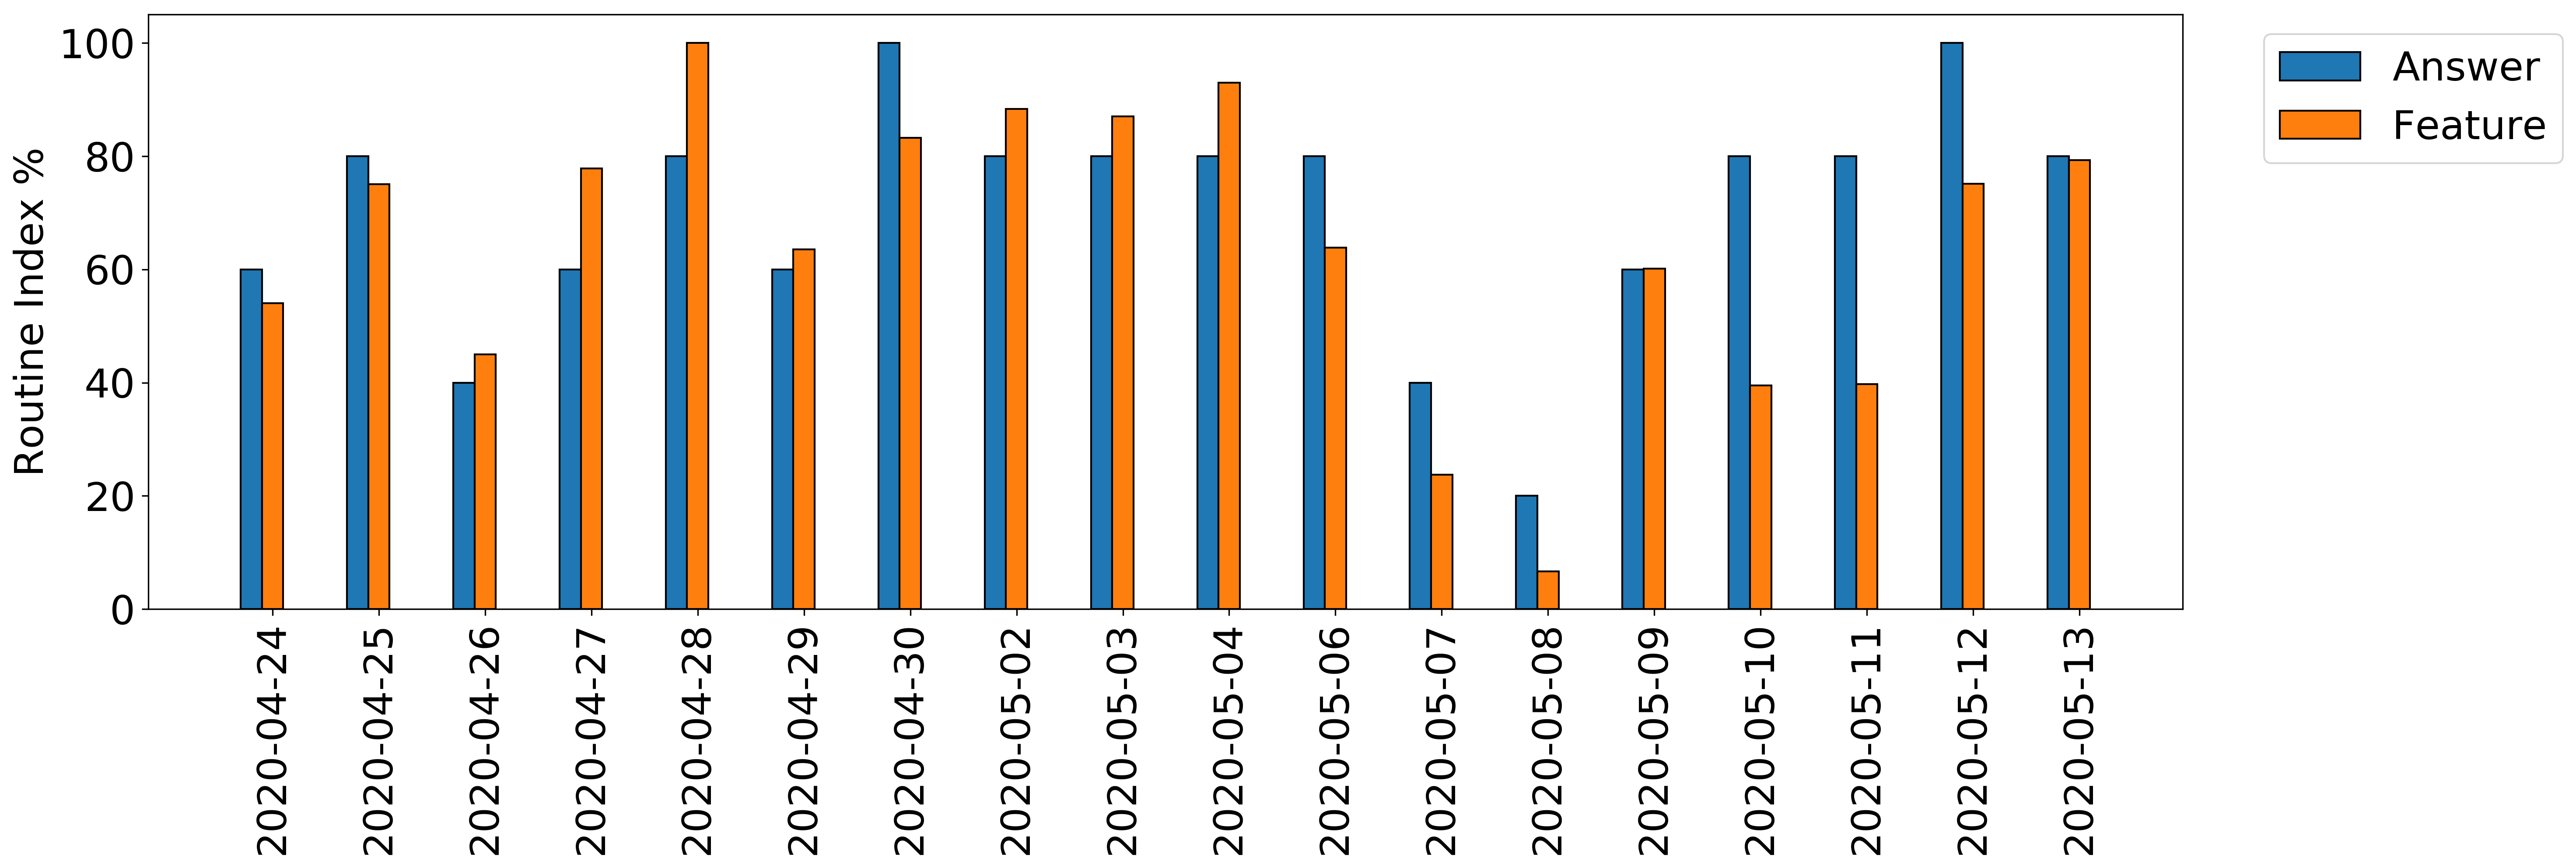
\includegraphics[0.5\textwidth]{images/study/routine_d6b2d9b9-398b-4e0d-b52b-224747f515c8.png}
    \caption{The answered and calculated data for each day, for the author}
    \label{fig:plot-daily}
\end{figure}

To say something about whether or not the algorithms undershoots or overshoots, the difference in sum was calculated as $ME = \frac{\sum(A) - \sum(F)}{N}$ ($N$ being the total number of days for the specific feature) meaning that if the result is positive then the answered result was on average higher and vice versa if the result is negative. The alternative is to calculate the mean error one can also calculate the mean of the difference per observation $ME = \frac{1}{N} \sum_{i=0}^{N} (a_i - f_i)$ however this the downside of cancelling out certain observations when the sign differs. 

The users generally answer that they have been at more places than the algorithms calculate.

Home stay generally predicts 10\% lower for half the participants, which was to be expected. Although for a couple of participants it predicts higher (i.e. negative mean error) although still within 10\% error. For participant 2 however it averages out to zero percent and for participant 1 the algorithms predict lower and has an error of 30\%.

The routine index is a mixed bag, with 6 participants answering higher than the algorithm and the remaining 4 being lower. All except for participant 6 deviating with almost 40\%. An important detail here is that the routine index was answered in increments of 20\% meaning that if a larger study was conducted in which the scale was more fine-grained, i.e. from 0 to 10 instead, it is possible the answers would be a lot closer to the predictions


\begin{figure}
    \centering
    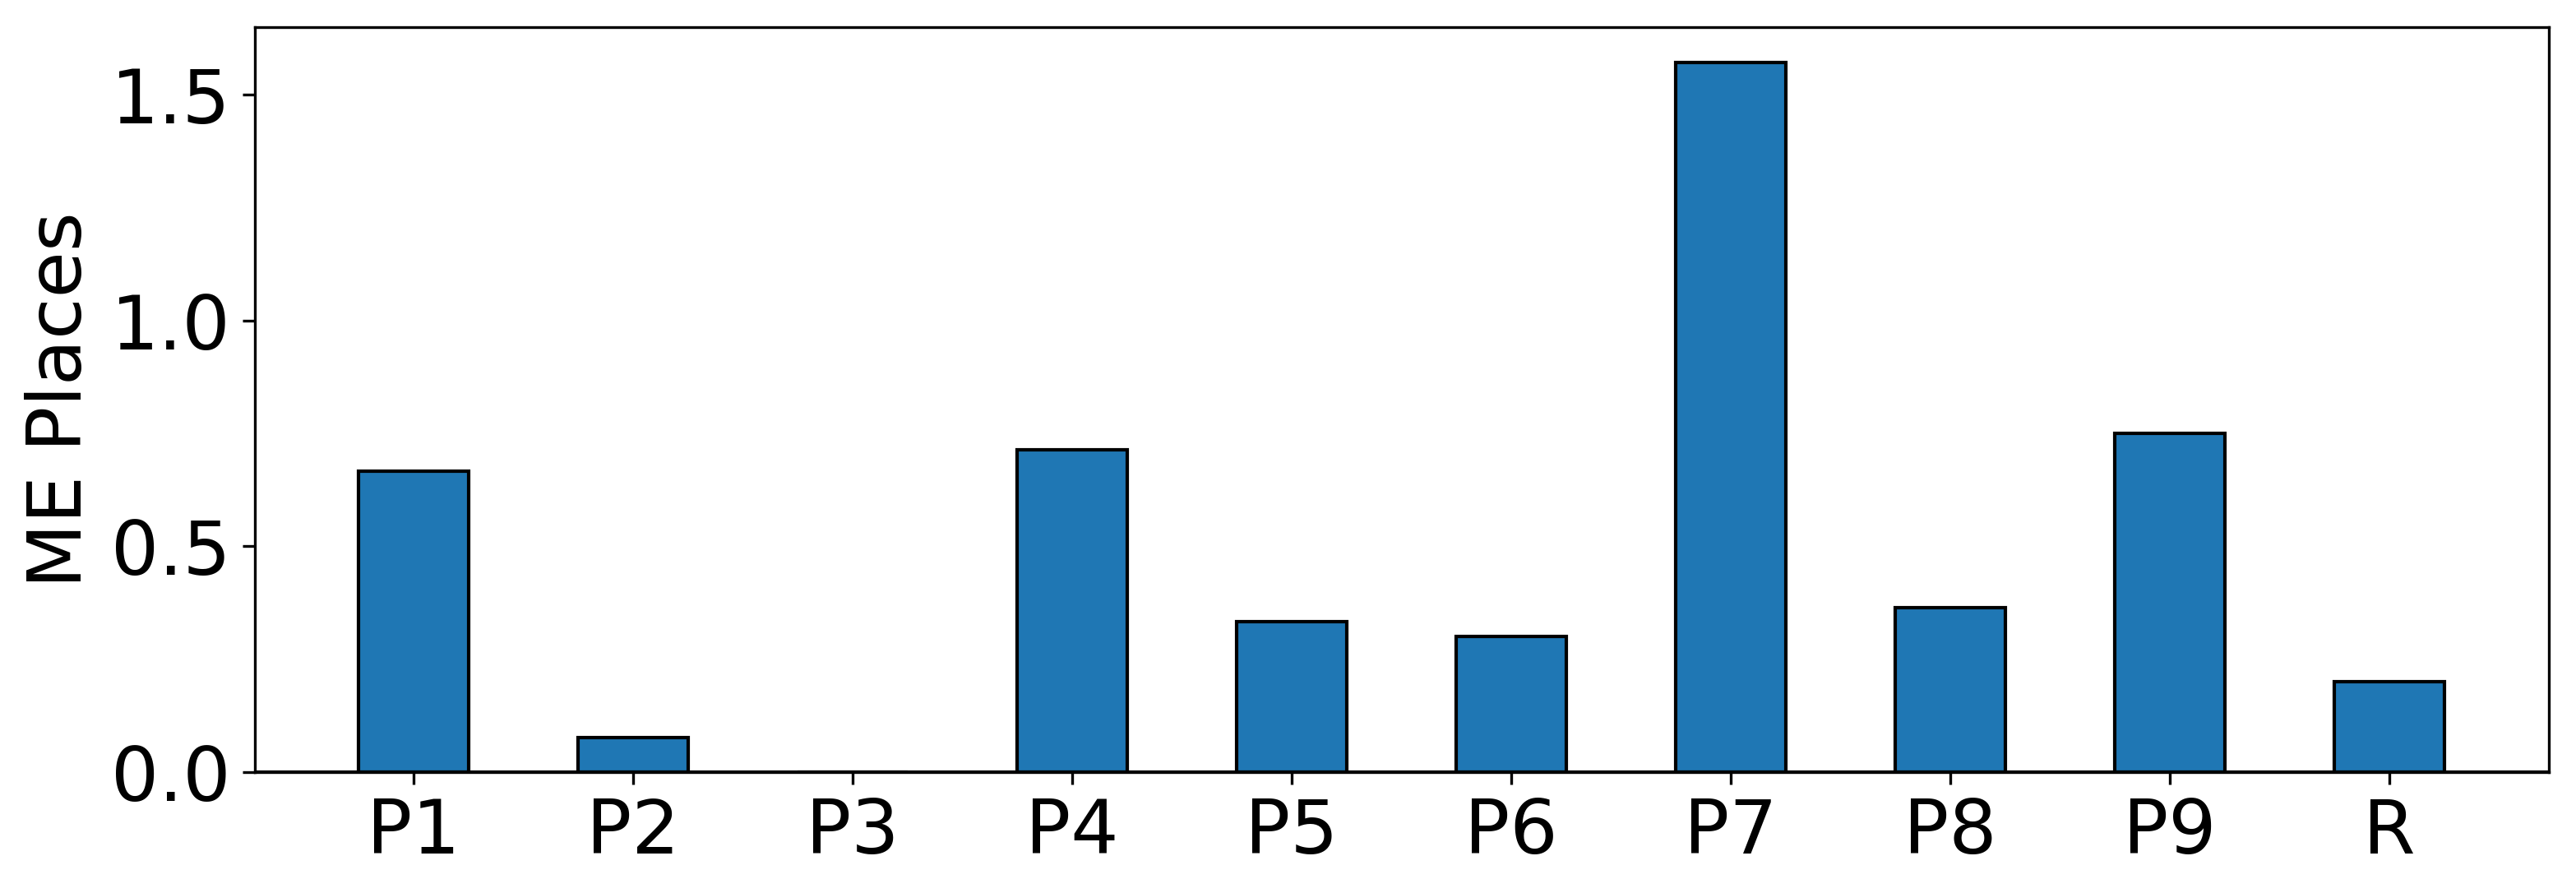
\includegraphics[0.5\textwidth]{images/study/me_places.png}
    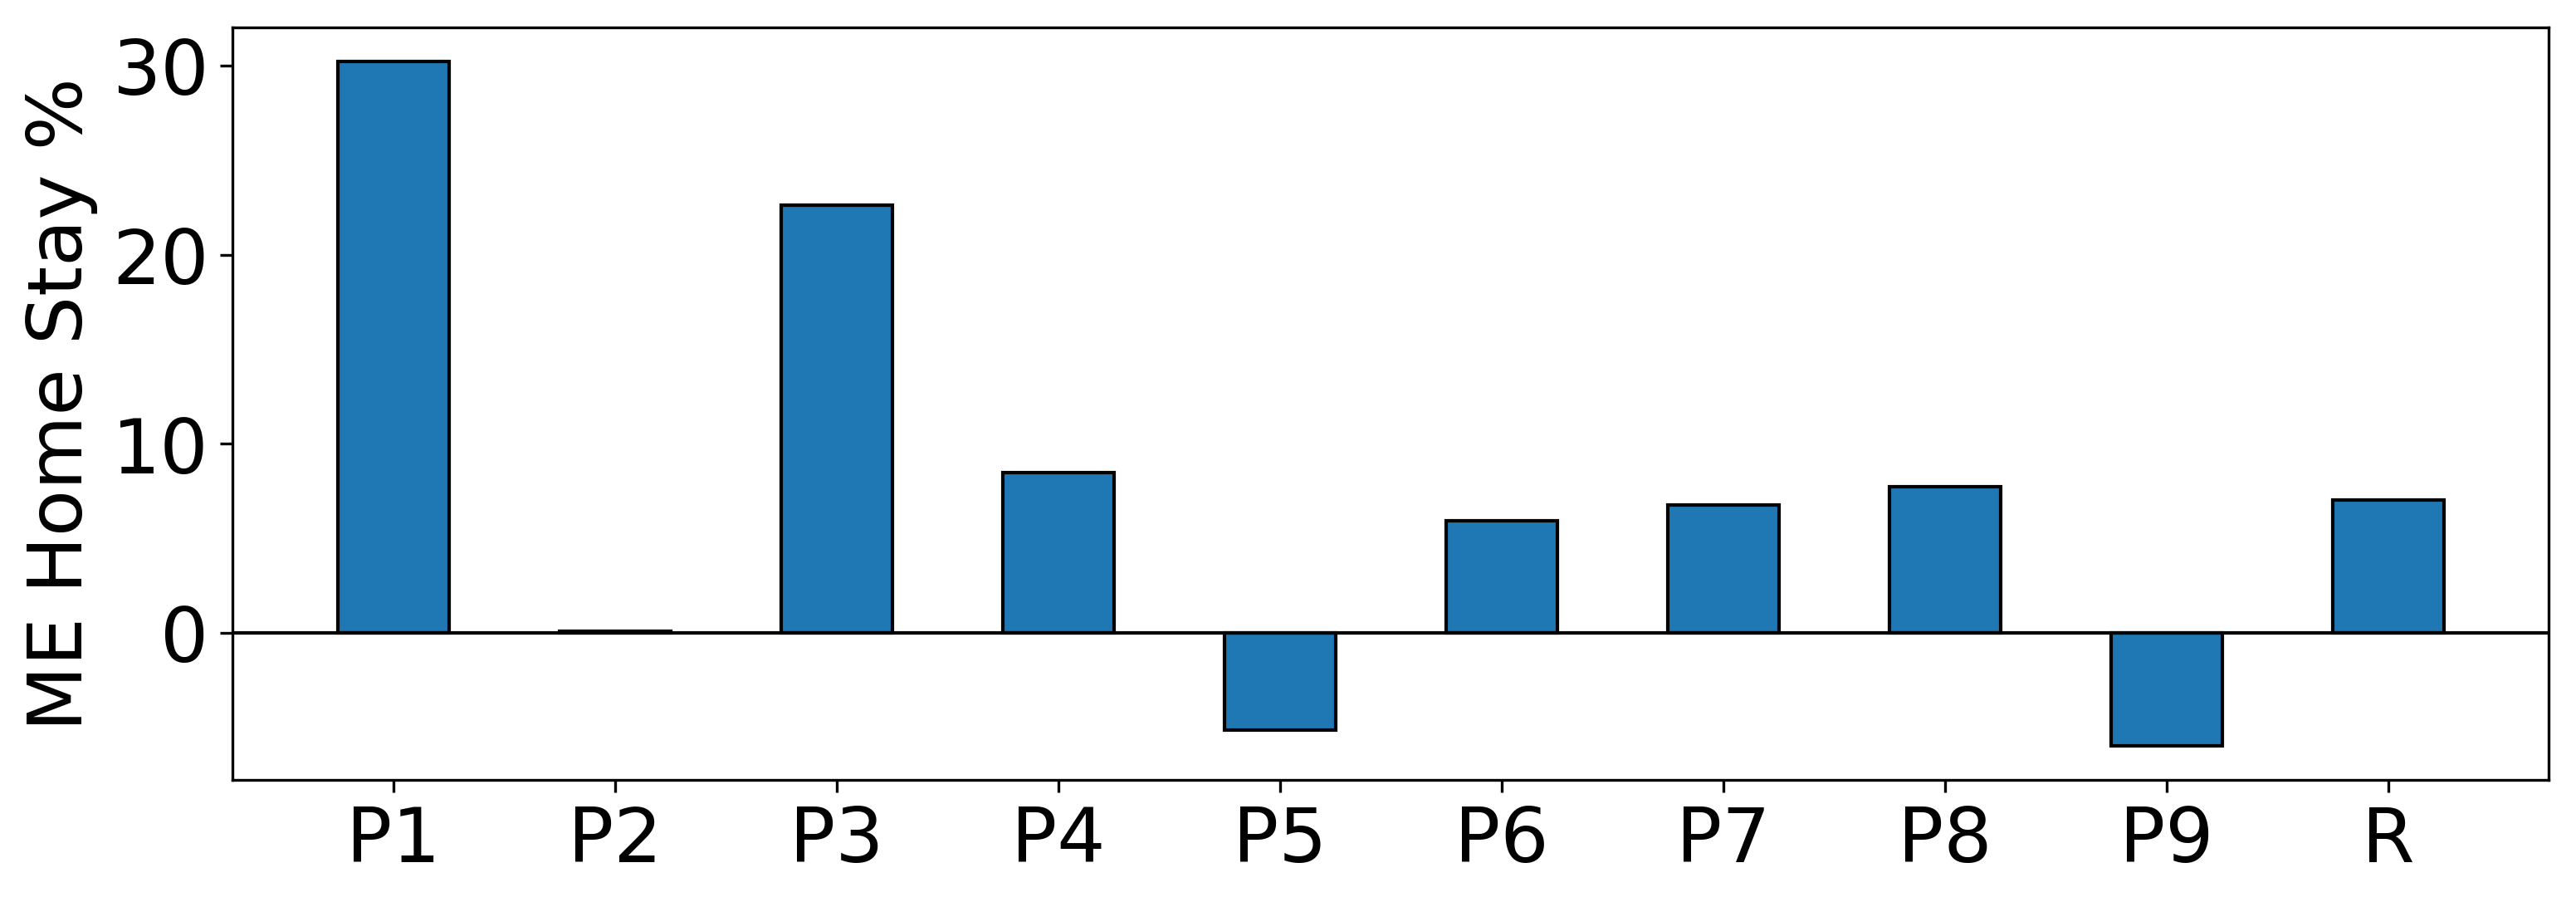
\includegraphics[0.5\textwidth]{images/study/me_homestay.png}
    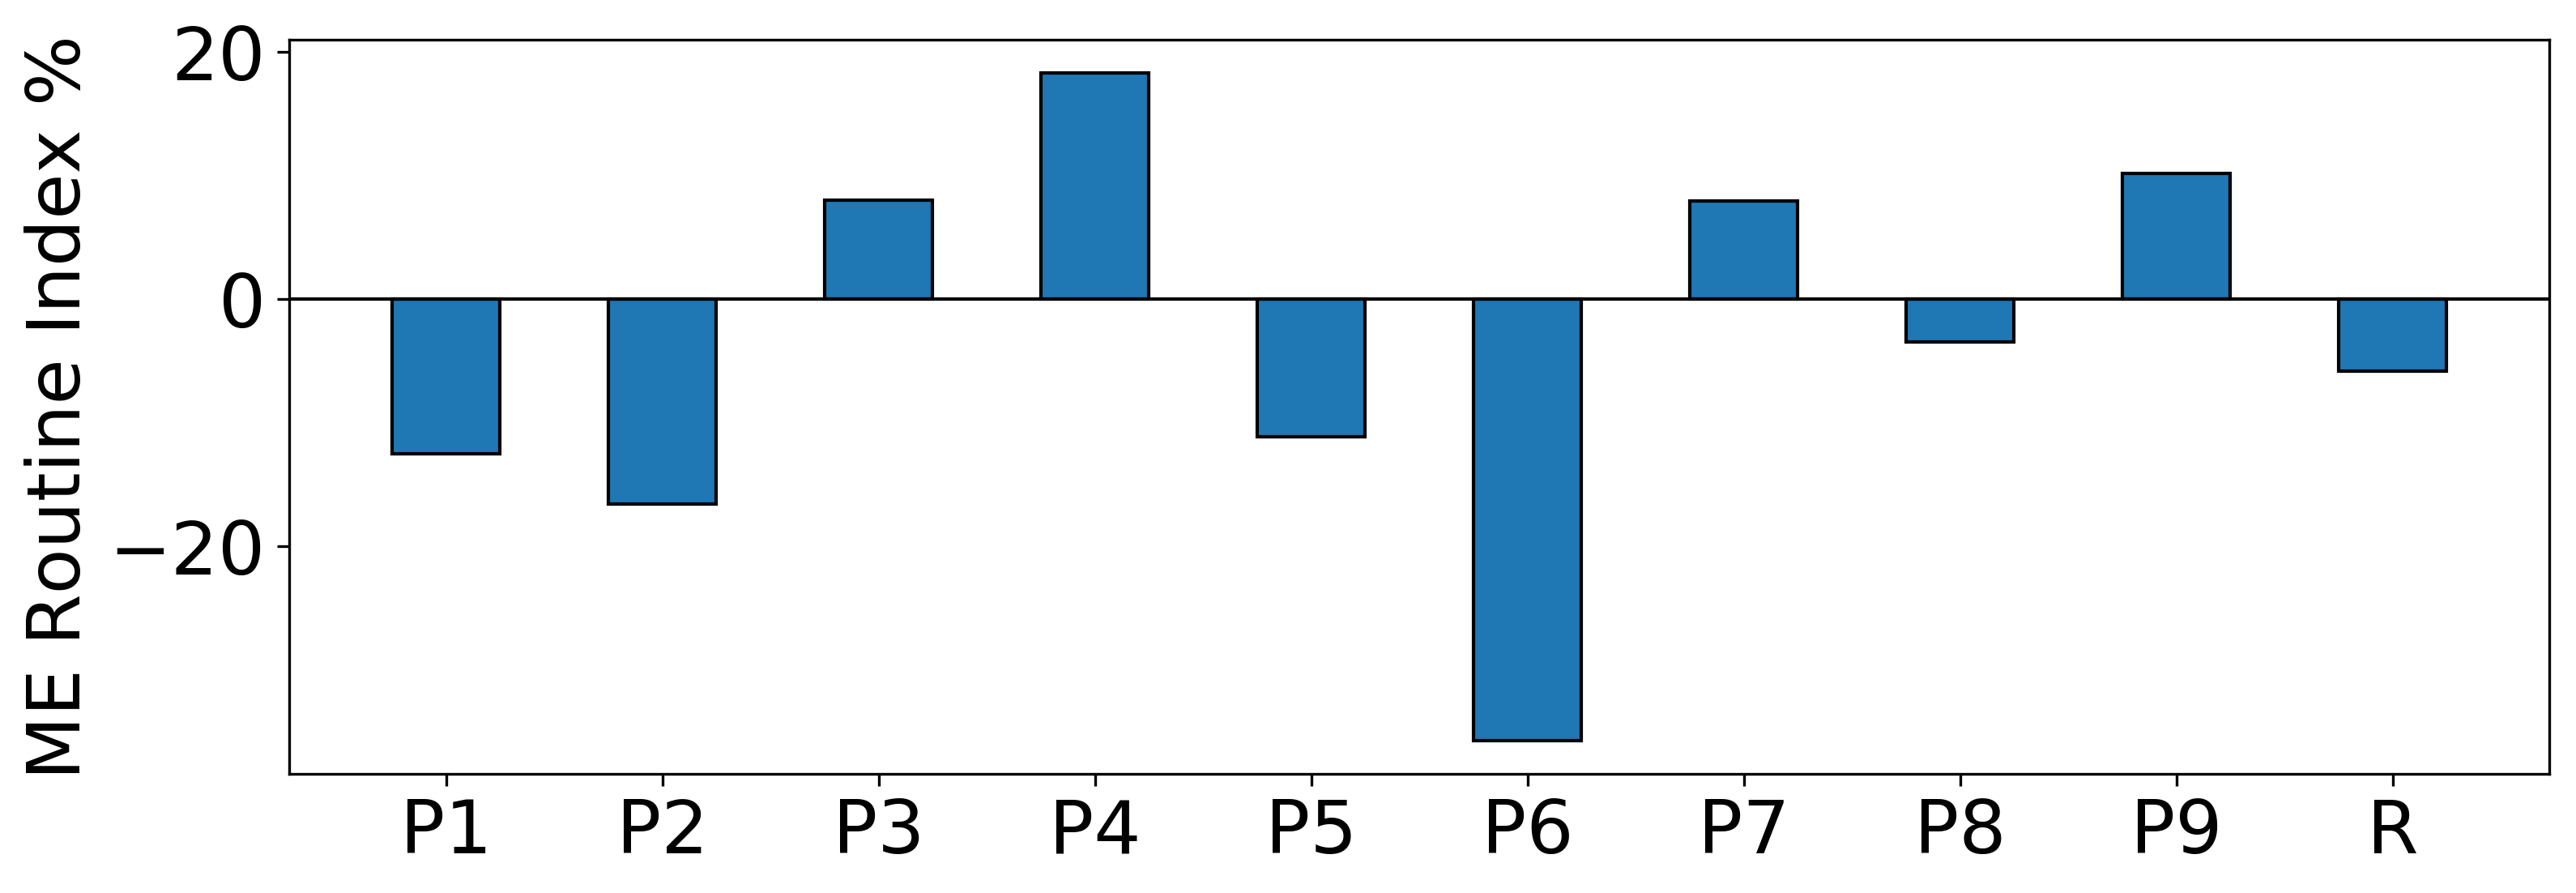
\includegraphics[0.5\textwidth]{images/study/me_routine.png}
    \caption{The number of data points in terms of days which could be evaluated, for each participant}
    \label{fig:plot-mean-error}
\end{figure}


